% PolyForge — M.Sc. thesis report
% Build: latexmk -pdf main.tex   (or: .\build.ps1)
% Every number in this document traces to a committed measurement record;
% see Appendix A and research/analysis/RESULTS_MASTER.md.

\documentclass[11pt,a4paper,oneside]{report}

\usepackage[T1]{fontenc}
\usepackage[utf8]{inputenc}
\usepackage{lmodern}
\usepackage{microtype}
\usepackage[margin=2.8cm]{geometry}
\usepackage{graphicx}
\usepackage{booktabs}
\usepackage{tabularx}
\usepackage{longtable}
\usepackage{amsmath,amssymb,amsthm}
\usepackage{xcolor}
\usepackage{caption}
\usepackage{setspace}
\usepackage{tikz}
\usetikzlibrary{arrows.meta,positioning,fit,calc}
\usepackage[numbers,sort&compress]{natbib}
\usepackage{xurl}
\usepackage[hidelinks]{hyperref}

\setlength{\emergencystretch}{2em}

\graphicspath{{../../eval/results/figures/}}

\newtheorem{proposition}{Proposition}
\captionsetup{font=small,labelfont=bf,width=0.92\textwidth}
\setstretch{1.12}

% ---- fill these in before submission -------------------------------------
\newcommand{\thesisauthor}{Mohaiminul}          % TODO: full legal name
\newcommand{\thesisdegree}{Master of Science}   % TODO: confirm degree title
\newcommand{\thesisuniversity}{[University]}    % TODO
\newcommand{\thesisdepartment}{[Department]}    % TODO
\newcommand{\thesissupervisor}{[Supervisor]}    % TODO
\newcommand{\thesisdate}{September 2026}
% ---------------------------------------------------------------------------

\newcommand{\polyforge}{PolyForge}
\newcommand{\jcac}{JCAC}
\newcommand{\dz}{d_z}
\newcommand{\evfile}[1]{\texttt{\small #1}}     % evidence-file pointer

\title{\polyforge{}: Joint Cross-Layer Control of Replicas, Semantic Cache,
and Model Tier for Multi-Tenant Hybrid Serving}
\author{\thesisauthor}
\date{\thesisdate}

\begin{document}

% ===== Title page ==========================================================
\begin{titlepage}
  \centering
  \vspace*{2cm}
  {\LARGE\bfseries \polyforge{}: Joint Cross-Layer Control of Replicas,\\
   Semantic Cache, and Model Tier\\
   for Multi-Tenant Hybrid Serving\par}
  \vspace{2cm}
  {\large A thesis submitted in partial fulfilment of the requirements\\
   for the degree of \thesisdegree\par}
  \vspace{2cm}
  {\Large \thesisauthor\par}
  \vspace{0.6cm}
  {\large \thesisdepartment\\ \thesisuniversity\par}
  \vspace{0.6cm}
  {\large Supervisor: \thesissupervisor\par}
  \vfill
  {\large \thesisdate\par}
\end{titlepage}

% ===== Abstract ============================================================
\begin{abstract}
\noindent
Multi-tenant platforms increasingly serve \emph{hybrid} workloads --- classic
CRUD traffic and AI inference from the same tenants on the same
infrastructure. The layers that govern the cost and quality of that serving
--- replica autoscaling, semantic response caching, and model-tier routing ---
are today controlled by independent, per-layer policies. This thesis argues,
and then measures, that per-layer local optima do not compose into a joint
optimum: a controller that plans \emph{replicas, semantic-cache budget, and
model tier together}, against one cost--SLO--fairness objective, dominates
tuned per-layer baselines.

\polyforge{} is that controller: a Kubernetes-native control plane with a
five-class workload taxonomy, an online classifier, a receding-horizon joint
planner (\jcac{}), and an operator that actuates plans under guardrails. The
evaluation is fully pre-registered --- seven protocols committed and pushed
before their first run --- with tuned baselines, paired seeds, effect sizes
with bootstrap confidence intervals, and published nulls.

As measured: on a 1{,}800-run blocked factorial matrix \polyforge{} beats
every tuned baseline (HPA, KEDA, FIRM-replica, GPTCache-LRU, static) on the
composite objective and on cost ($|\dz|$ 0.66--1.44); on replayed real demand
(BurstGPT, 10.63M requests) the powered confirmatory replay ($n{=}96$) shows
$-70\%$ cost against tuned HPA/KEDA/FIRM ($p \le 4.3\times10^{-6}$) with a
disclosed $+0.07$ violation trade; on real LMSYS-Chat-1M prompts the adaptive
semantic cache reaches 29.6\% hit rate at cosine $0.85$ ($+93\%$ over a
non-strawman fixed baseline) with hit \emph{precision} measured rather than
assumed; fairness beats both a FIRM-style and a VTC-style baseline on Jain's
index at lower cost; and a timing side channel in shared semantic caches is
demonstrated (AUC 0.88) and closed by per-tenant partitioning at 24\% latency
cost, dominating padding and TTL-jitter defenses. Two pre-registered SLO
hypotheses failed and are published as failures; the honest SLO claim is
violation \emph{parity} with tuned reactive scalers at 43--48\% lower cost.
All headline numbers are decision-quality measurements under a stated system
model, calibrated against a real inference server and a real GPU tier bench.
Live-cluster validation is ordinal-only by design; both arms are
live-verified end to end, and the pre-registered ordinal check is reported
as measured: at the replica-only live projection the two controllers tie,
and the simulator's ranking does not reproduce --- a published
disagreement whose mechanisms (the inert live cache lever, disclosed
pre-run, and a measured sim-side overestimate of reactive lateness) are
analyzed in the evaluation.
\end{abstract}

\tableofcontents
\listoffigures
\listoftables

% ===== Chapters ============================================================
\chapter{Introduction}
\label{ch:introduction}

\section{The problem: hybrid serving is controlled one layer at a time}

Multi-tenant platforms no longer serve one kind of traffic. The same tenants,
on the same clusters, issue classic CRUD requests and AI inference requests
--- chat completions, embeddings, multi-step agent chains --- often within a
single user-facing transaction. Three control surfaces govern what that
serving costs and how it feels:

\begin{enumerate}
  \item \textbf{Replica autoscaling} decides how much capacity each service
        holds. In production this is the Kubernetes Horizontal Pod Autoscaler
        (HPA)~\citep{k8shpa}, KEDA~\citep{keda}, or a research
        controller~\citep{firm2020,sageserve2025,chiron2025,aladdin2024}.
  \item \textbf{Semantic response caching} decides which AI answers are
        served from an embedding-similarity cache instead of a model
        call~\citep{gptcache2023,scalm2024,instcache2024,meancache2024}.
  \item \textbf{Model-tier routing} decides which of several differently
        priced model classes answers each request~\citep{infaas2019}.
\end{enumerate}

Each layer has a mature literature and, in every surveyed system, an
independent controller: an autoscaler that has never heard of the cache, a
cache that does not know what a replica costs, a router that optimizes one
request at a time. Each controller can be locally optimal. This thesis starts
from the observation that the three layers share one budget, one latency
target, and one set of tenants --- and asks whether local optima compose.

\section{Thesis statement}

\begin{quote}
\emph{Per-layer local optima do not compose into a joint optimum. A
controller that plans replicas, semantic-cache budget, and model tier
together --- one receding-horizon optimization per control interval, against
a single objective in cost, SLO compliance, and cross-tenant fairness ---
dominates tuned per-layer baselines on that objective, and does so with
per-tenant dollar accounting and budget guardrails that no surveyed system
provides.}
\end{quote}

The claim is tested, not asserted: against five baselines each grid-tuned on
the thesis's own objective, under pre-registered protocols (seven at the
first campaign, forty-eight by the last) whose hypotheses --- including the
ones that failed --- were committed and pushed before the first run.

\section{What was built}

\polyforge{} is a Kubernetes-native control plane implementing the thesis
statement end to end (Chapter~\ref{ch:design}):

\begin{itemize}
  \item a \textbf{control plane} (Go) for tenants, projects, API keys, rate
        limits, and telemetry, with row-level-security-enforced tenant
        isolation proven by test;
  \item an \textbf{AI gateway} (Go) with multi-backend chat routing, a
        semantic cache with cost-aware eviction, vector search, and an agent
        loop;
  \item a \textbf{workload classifier} mapping 12-feature telemetry windows
        onto a five-class taxonomy with drift detection;
  \item the \textbf{\jcac{} planner} (\emph{Joint Cache--Autoscaling
        Control}): receding-horizon model-predictive control over a
        move-blocked action lattice, minimizing
        $J = \alpha\,\text{cost} + \beta\,\text{SLO violation} +
        \gamma\,(1-\text{Jain})$, deployed as a Python service that imports
        the simulator's controller so offline and online planning are the
        same code;
  \item a \textbf{Kubernetes operator} (Go) with four CRDs (Tenant,
        WorkloadProfile, Policy, Budget) that actuates plans under
        guardrails: replica bounds, one cache level per step, per-tenant
        budget caps, and last-good-plan fallback.
\end{itemize}

\section{Contributions}

\begin{enumerate}
  \item \textbf{Joint cross-layer control.} The first surveyed controller to
        co-optimize replicas, semantic-cache budget, and model tier against
        one multi-tenant objective (Chapter~\ref{ch:design}); ablating
        jointness worsens the objective's cost term --- by $+2884\%$ against
        the published layered comparator, and by a margin $86\%$ smaller
        once that comparator's absorbing-tier defect is repaired
        (Section~\ref{sec:eval-v1}); the smaller number is the claim.
  \item \textbf{A measured composition result, and its adjudication.} On a
        1{,}800-run blocked factorial with tuned baselines, \polyforge{} wins
        the composite objective against every baseline ($|\dz|$ 0.66--1.44)
        and is the only Pareto-undominated system --- non-dominated in 48 of
        60 cells under \emph{any} weighting; the composite-$J$ win holds in
        every later campaign that tested it, including against an
        offline-trained learned joint controller over the same action space.
        The \emph{cost} component was then re-scored against comparators
        corrected for three confounds found after the campaigns closed
        (Section~\ref{sec:eval-adjudication}): the replayed-BurstGPT $-70\%$
        and Azure $-42\%$ headlines are \textbf{withdrawn} as like-for-like
        comparisons, and what survives is a feasibility result --- the
        per-tenant budget is satisfiable only by a controller holding the
        tier knob, and no replica-only reactive controller can meet it under
        AI load by any decision available to it.
  \item \textbf{An honest SLO result.} Two pre-registered attempts to beat
        tuned reactive scalers on raw violation failed and are published as
        failures; what holds is violation parity at $-43$\ldots$-48\%$ cost,
        a confirmed forecasting mechanism (seasonal $<$ trend on violation
        where real periodicity exists, $p=6\times10^{-4}$), and a
        declared-exploratory win in the spike regime where reaction is
        structurally impossible (Section~\ref{sec:eval-v3}). On the
        unbounded severity metric the synthetic and Azure advantage is real
        and the BurstGPT one reverses; both are stated together, always.
  \item \textbf{Real-data cache results with a quality denominator.} On real
        LMSYS-Chat-1M prompts: 29.6\% adaptive hit rate at cosine 0.85
        ($+93\%$ over a 10\%-of-working-set fixed cache), dollar-weighted
        savings, an empirical hit-rate--capacity curve, and --- unique among
        surveyed cache papers --- measured hit \emph{precision} with its
        stochasticity ceiling (Section~\ref{sec:eval-cache}).
  \item \textbf{Fairness at the control-plane altitude.} Beats a FIRM-style
        baseline on Jain's index ($\dz{=}1.0$) and a VTC-style replica-level
        transplant \emph{on Jain itself} at $-35\%$ cost; the controller's
        own fairness term is honestly nulled under injected interference
        (Section~\ref{sec:eval-fairness}).
  \item \textbf{A security frontier for shared semantic caches.} A timing
        side channel leaking prompt membership at AUC 0.88, and a defense
        comparison in which per-tenant partitioning restores
        attacker-to-chance at 24\% latency cost, dominating padding and TTL
        jitter (Section~\ref{sec:eval-security}).
  \item \textbf{Construction-level theory.} Block-coordinate optimality of
        the planner's two-sweep solver and boundedness/contraction of its
        self-calibration scale, stated at exactly the altitude the code
        delivers (Section~\ref{sec:design-theory}); a single-tenant cost
        separation between reactive and predictive control computed from
        the plant constants alone, shown to be exactly the information
        asymmetry of observational aliasing; and its multi-tenant extension
        computed exactly and \emph{falsified} against the measured arms
        (Section~\ref{sec:eval-summary}).
  \item \textbf{Live evidence at three depths.} A replica-only ordinal check
        on a kind cluster (disagreement, published), a valid 24-hour soak
        (25.8M requests, nothing dropped, two of four hypotheses failed and
        published), a real trace driving the real cluster, and a three-knob
        live plane on a rented GPU host on which the published controller
        \emph{lost} to its own ablation, the corrected controller then beat
        every arm at iso-fairness, and the obvious damper for its
        oscillation failed (Section~\ref{sec:eval-live}).
  \item \textbf{A pre-registered systems methodology.} Forty-eight
        protocols pushed before their runs, tuned baselines, paired effect
        sizes with bootstrap CIs, stopping rules, substrate separation, an
        adjudication practice in which confounds found after a campaign
        closes are answered by a new pre-registered record and never by
        editing the old one, and a published honest-nulls ledger
        (Chapter~\ref{ch:methodology}) --- a methodological contribution
        independent of any performance number.
\end{enumerate}

\section{Scope and honesty of claims}
\label{sec:intro-scope}

Every headline number in this thesis is \emph{decision quality under a stated
system model}: a discrete-event simulator whose congestion form was
calibrated against a real inference server (the fit direction errs
\emph{against} \polyforge{}'s lean postures) and whose model-tier constants
were checked against a real GPU latency bench. Real data enters three ways:
replayed BurstGPT demand (10.63M requests) and Azure LLM inference 2024
demand (44.1M requests) for the cost and forecasting claims, and real
LMSYS-Chat-1M prompts for the cache claims. Live-cluster validation never
compares absolutes across substrates. The replica-only ordinal check
recorded a \emph{disagreement} (live parity between the arms), published as
measured; the three-knob live plane that followed on a rented GPU host is
the one place where every knob is live and every arm is scored on the same
cells, and its verdicts --- the published controller's loss, the corrected
controller's win, the damper's failure --- are reported in
Section~\ref{sec:eval-live} exactly as their frozen protocols scored them.
What is \emph{not} claimed: any comparative cost percentage against the
originally tuned baselines (withdrawn, Section~\ref{sec:eval-adjudication}),
absolute dollar or latency numbers transferring to any production fleet,
token-level scheduling fairness, or tail behavior beyond p95 on the
simulated substrate.

\section{Document structure}

Chapter~\ref{ch:background} positions the work against autoscaling, caching,
fairness, and the 2026 serving stack. Chapter~\ref{ch:design} presents the
architecture, the \jcac{} formulation, and the two propositions.
Chapter~\ref{ch:implementation} covers the implementation and its
engineering gates. Chapter~\ref{ch:methodology} defines the pre-registered
methodology. Chapter~\ref{ch:evaluation} reports all campaigns ---
wins, nulls, and failures. Chapter~\ref{ch:discussion} confronts threats to
validity. Chapter~\ref{ch:conclusion} concludes.
Appendix~\ref{app:traceability} maps every claim to its committed evidence.

\chapter{Background and Related Work}
\label{ch:background}

This chapter positions \polyforge{} against four bodies of work: autoscaling
for inference serving, semantic caching, multi-tenant fairness, and the
production LLM-serving stack of 2025--26. One reading rule applies
throughout, and it is the same rule the evaluation enforces
(Chapter~\ref{ch:methodology}): \textbf{numbers from other papers are their
numbers on their substrate} --- real GPU fleets, their traces, their
baselines --- while \polyforge{}'s numbers are decision quality on its own
matrix and traces. No comparison in this chapter is a head-to-head cell; the
comparison is \emph{shape against shape}. Where a published system is
reproducible at simulator scale, \polyforge{} carries it as a tuned in-matrix
baseline instead (HPA, KEDA, FIRM-replica, GPTCache-LRU, static, and iso-cost
variants).

\section{Autoscaling for inference serving}

The Kubernetes Horizontal Pod Autoscaler~\citep{k8shpa} and
KEDA~\citep{keda} are the production defaults: reactive controllers on
utilization or event-lag signals. FIRM~\citep{firm2020} added fine-grained,
SLO-oriented resource management for microservices.

The LLM-serving generation is forecast-aware and hierarchical.
SageServe~\citep{sageserve2025} reports ${\sim}25\%$ GPU-hour savings on 10M
production requests using demand forecasting; Chiron~\citep{chiron2025}
reports up to $+90\%$ SLO attainment and $+70\%$ GPU efficiency via
hierarchical autoscaling; Aladdin~\citep{aladdin2024} jointly places and
scales for up to $-71\%$ serving cost; an SLO-driven Kubernetes autoscaler
\citep{k8sslo2025} reports $-31\%$ violation duration at $-18\%$ cost.
Joint horizontal-plus-vertical scaling~\citep{taleoftwoscales2024} and
SLO-constrained joint allocation~\citep{jointalloc2026} widen a single
layer's action space; INFaaS~\citep{infaas2019} pioneered model-variant
selection (``model-less'' serving); Faro~\citep{faro2024} targets on-premise
inference clusters.

Two observations motivate this thesis. First, the closest systems to
``joint'' --- Aladdin (placement$+$scaling), the horizontal$+$vertical
scalers, INFaaS-style variant selection --- each co-optimize \emph{within}
one layer. None of them controls a semantic cache, and none carries
cross-tenant fairness in its objective. Second, the published wins are
typically measured against default or non-SLO-tuned baselines; the bar in
this thesis is deliberately higher --- every baseline is grid-tuned on the
paper's own objective (Section~\ref{sec:method-baselines}).

\section{Semantic caching for LLM serving}

GPTCache~\citep{gptcache2023} established the pattern --- embed the prompt,
serve a stored response on similarity --- reporting 61.6--68.8\% hit rates on
its own benchmark. SCALM~\citep{scalm2024} reports $+63\%$ hits over
GPTCache; InstCache~\citep{instcache2024} pre-populates predicted
instructions and reports 51.34\% on LMSYS-Chat-1M;
MeanCache~\citep{meancache2024} moves the cache user-side and federated;
\citet{semcacheadapt2025} study offline-to-online adaptation of similarity
thresholds.

In all of these, \emph{the cache is the system}: its size is an input, not a
decision variable, and its interaction with capacity and model choice is out
of scope. \polyforge{} treats cache budget as one of three jointly planned
knobs, prices its benefit per tenant in dollars, and adds two measurements
the cache literature does not publish: hit \emph{precision} against the
actually received response on the same real dataset
(Section~\ref{sec:eval-cache}), and a timing side-channel analysis with a
defense frontier (Section~\ref{sec:eval-security};
cf.~the prompt-cache audit of \citet{promptcacheaudit2025}).

\section{Multi-tenant fairness}

VTC~\citep{vtc2024} defined service fairness for LLM serving at token
granularity inside a continuous-batching engine, with a proven $2\times$
service bound; Equinox~\citep{equinox2025}, D\textsuperscript{2}LPM
\citep{d2lpm2025}, and Justitia~\citep{justitia2025} extend it (worst-case
service gaps $-42\%$ vs.\ VTC; locality; efficiency). \polyforge{}'s fairness
sits at a different altitude --- capacity allocation across tenants at the
control-plane level, scored by Jain's index~\citep{jain1984} over per-tenant
SLO satisfaction --- and the claims are scoped to that altitude
(Section~\ref{sec:disc-fairness-altitude}). The evaluation carries a
replica-level transplant of VTC's least-service-first idea as a tuned
baseline (\evfile{vtc\_replica}); beating it on Jain says \polyforge{}
allocates capacity more evenly, not that it schedules tokens more fairly.
Token-level fair schedulers are complementary: they would run \emph{inside}
each replica pool \polyforge{} sizes.

\section{The 2026 serving substrate, and where \polyforge{} sits}
\label{sec:bg-substrate}

The production stack of 2025--26 --- llm-d~\citep{llmd2025},
AIBrix~\citep{aibrix2025}, NVIDIA Dynamo~\citep{dynamo2025}, and the
Kubernetes Gateway API Inference Extension~\citep{gatewayapi2025} ---
actuates on signals \polyforge{}'s system model does not name: queue depth,
in-flight requests, KV-cache pressure, prefill/decode pool split. That is an
altitude difference, not a contradiction. \polyforge{} is the
\emph{portfolio} controller above that actuation layer, and each knob has a
direct target in it:

\begin{table}[htbp]
\centering\small
\begin{tabular}{@{}lll@{}}
\toprule
\textbf{\polyforge{} knob} & \textbf{In the system model} & \textbf{2026 actuation target} \\
\midrule
replicas   & per-tenant capacity      & decode-pool size / vLLM pod count \\
cache MB   & semantic-cache budget    & gateway semantic-cache budget \\
tier       & model class (1:10:100)   & model routing (INFaaS-style; AIBrix) \\
\bottomrule
\end{tabular}
\caption{Substrate mapping of \polyforge{}'s three knobs onto the 2026
LLM-serving stack (from \evfile{docs/RELATED\_WORK.md}~\S4).}
\label{tab:substrate-mapping}
\end{table}

Two design decisions keep the mapping honest: the demand signal sits behind
an interface (\evfile{planner.DemandSource}), so a token-level source (TTFT,
queue depth, KV pressure) replaces the request-rate source without touching
the planner; and latency claims stay request-level, scoped away from
continuous-batching token dynamics. What the 2026 stack does \emph{not} do
--- and where \polyforge{} sits --- is decide jointly, across a tenant
portfolio, in dollars, with per-tenant budget guardrails.

\section{Capability gap summary}

Across all surveyed systems, none co-optimizes replicas, semantic cache, and
model tier against one multi-tenant objective; none accounts per-tenant
dollars with budget guardrails; none publishes a security evaluation of its
cache layer; and none pre-registers its hypotheses or publishes its nulls.
Those four rows --- one architectural, one economic, one adversarial, one
methodological --- are the thesis's position in the literature. The full
capability matrix, including the rows where surveyed systems dominate
\polyforge{} (live GPU fleets, production scale, proven scheduling bounds),
is maintained in \evfile{docs/RELATED\_WORK.md} and summarized honestly in
Section~\ref{sec:disc-limits}.

\chapter{System Design}
\label{ch:design}

\polyforge{} is an adaptive control plane for multi-tenant clusters serving
hybrid workloads. This chapter walks the control loop end to end
(Figure~\ref{fig:architecture}), then presents the \jcac{} formulation and
the two construction-level guarantees the deployed solver carries.

\section{The control loop, end to end}
\label{sec:design-loop}

\begin{figure}[htbp]
\centering
\resizebox{0.99\linewidth}{!}{%
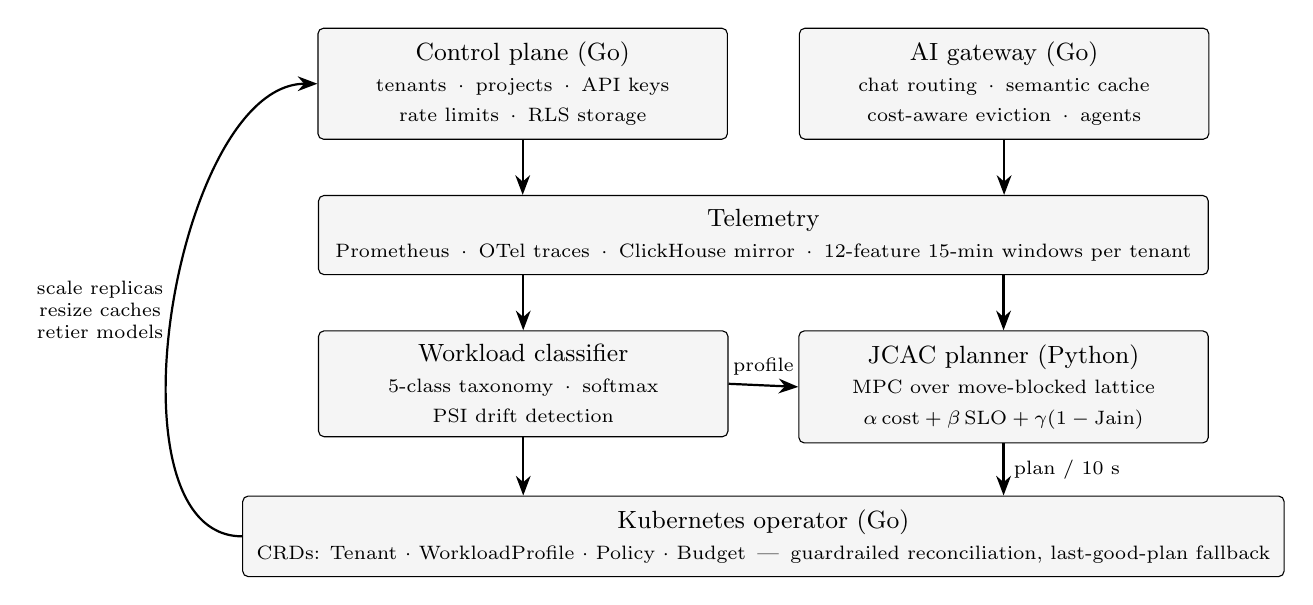
\begin{tikzpicture}[
  box/.style={draw, rounded corners=2pt, align=center, font=\small,
              minimum height=9mm, inner sep=5pt, fill=gray!8},
  arr/.style={-{Stealth[length=2.5mm]}, thick},
  node distance=7mm and 9mm
]
\node[box, minimum width=52mm] (cp)
  {Control plane (Go)\\ \scriptsize tenants \,$\cdot$\, projects \,$\cdot$\, API keys\\
   \scriptsize rate limits \,$\cdot$\, RLS storage};
\node[box, minimum width=52mm, right=of cp] (gw)
  {AI gateway (Go)\\ \scriptsize chat routing \,$\cdot$\, semantic cache\\
   \scriptsize cost-aware eviction \,$\cdot$\, agents};
\node[box, minimum width=113mm, below=of $(cp.south)!0.5!(gw.south)$] (tel)
  {Telemetry\\ \scriptsize Prometheus \,$\cdot$\, OTel traces \,$\cdot$\, ClickHouse mirror
   \,$\cdot$\, 12-feature 15-min windows per tenant};
\node[box, minimum width=52mm, below=of tel.south west, anchor=north west] (clf)
  {Workload classifier\\ \scriptsize 5-class taxonomy \,$\cdot$\, softmax\\
   \scriptsize PSI drift detection};
\node[box, minimum width=52mm, below=of tel.south east, anchor=north east] (plan)
  {\jcac{} planner (Python)\\ \scriptsize MPC over move-blocked lattice\\
   \scriptsize $\alpha\,\mathrm{cost}+\beta\,\mathrm{SLO}+\gamma(1-\mathrm{Jain})$};
\node[box, minimum width=113mm, below=7mm of $(clf.south)!0.5!(plan.south)$] (op)
  {Kubernetes operator (Go)\\ \scriptsize CRDs: Tenant $\cdot$ WorkloadProfile $\cdot$
   Policy $\cdot$ Budget \,---\, guardrailed reconciliation, last-good-plan fallback};
\draw[arr] (cp.south) -- (tel.north -| cp.south);
\draw[arr] (gw.south) -- (tel.north -| gw.south);
\draw[arr] (tel.south -| clf.north) -- (clf.north);
\draw[arr] (clf.east) -- node[above,font=\scriptsize]{profile} (plan.west);
\draw[arr] (tel.south -| plan.north) -- (plan.north);
\draw[arr] (plan.south) -- node[right,font=\scriptsize]{plan / 10 s} (op.north -| plan.south);
\draw[arr] (clf.south) -- (op.north -| clf.south);
\draw[arr] (op.west) .. controls +(-18mm,0) and +(-18mm,0) .. node[left,font=\scriptsize,align=center]{scale replicas\\ resize caches\\ retier models} (cp.west);
\end{tikzpicture}%
}
\caption{The \polyforge{} control loop. Requests (CRUD $+$ AI, JWT-scoped per
tenant) hit the control plane and AI gateway; per-request telemetry is
aggregated into per-tenant feature windows; the classifier labels each
tenant's workload; every 10\,s the \jcac{} planner emits a joint plan
(replicas, cache budget, model tier per tenant); the operator actuates it
under guardrails against the same data plane the requests hit.}
\label{fig:architecture}
\end{figure}

\paragraph{Control plane.} Tenant, project, and API-key management; rate
limiting; telemetry ingestion. Tenant isolation is enforced by PostgreSQL
row-level security \emph{at the database}, not in the query builder, and is
proven by a test that queries the telemetry table with no tenant predicate
inside a tenant transaction context and asserts foreign rows are invisible
(ADR 0003).

\paragraph{AI gateway.} Multi-backend chat routing by plan, length, and
budget; a semantic cache with \textbf{cost-aware eviction} (evict by
expected re-computation dollars, not recency alone); vector search; an agent
loop. The cache is per-tenant by default --- a security decision, not only a
fairness one (Section~\ref{sec:eval-security}).

\paragraph{Telemetry and classification.} Every request lands in Prometheus
metrics, OpenTelemetry traces, and an analytical mirror. Per tenant, a
15-minute window is reduced to a 12-feature vector (rates, mix, burstiness,
latency percentiles, cache affinity); a softmax classifier maps windows onto
a five-class taxonomy --- steady CRUD, bursty CRUD, cacheable AI chat,
uncacheable AI chat, agentic --- with population-stability-index drift
detection. Each class carries a control implication (e.g., agentic latency
needs the tier knob, not more replicas), which the evaluation makes
measurable (Figure~\ref{fig:violation-by-workload}).

\paragraph{\jcac{} planner.} A receding-horizon model-predictive controller
over a \emph{move-blocked action lattice} (Section~\ref{sec:design-jcac}).
The deployed Python service imports the simulator's controller module ---
offline evaluation and online planning are provably the same code, which is
what licenses reading simulator decision quality as deployed decision
quality (Section~\ref{sec:disc-validity}).

\paragraph{Operator.} Four CRDs --- Tenant, WorkloadProfile, Policy, Budget
--- reconciled with guardrails: replica bounds, at most one committed cache
level move per step, per-tenant budget caps, ordered finalizer teardown, and
last-good-plan fallback when the planner is unreachable or over deadline.
When several Policies resolve to one shared target, their clamped
contributions are \emph{summed} (pool-tenant semantics) rather than
last-writer-wins --- a correctness property found and fixed at the desk
before the live campaign (Section~\ref{sec:impl-live}).

\section{The \jcac{} formulation}
\label{sec:design-jcac}

At each control step the planner holds tenants $T=\{1,\dots,m\}$. Tenant
$i$'s decision variable is $x_i=(r_i,c_i,\tau_i)$ --- replicas, cache level,
model tier --- drawn from a finite per-tenant lattice $X_i$: replica deltas
$\Delta r\in\{-2,\dots,2\}$, cache moves at most one committed level, tier
$\tau_i\in\{\text{none},\text{small},\text{mid},\text{large}\}$; hence
$|X_i|\le 60$ and the joint space $X=\prod_i X_i$ is finite. The per-step
objective is
\begin{equation}
\label{eq:objective}
\begin{split}
J(x)={}&\alpha\frac{1}{S}\sum_{i}\mathrm{cost}_i(x_i)
      +\beta\sum_{i}\mathrm{obj}_i(x_i)
      +\gamma\sum_{i}w_i\bigl(1-\mathrm{Jain}(s(x))\bigr)\\
      &+\gamma\sum_i \nu_i\,\rho_i(x_i)
      +\lambda\sum_i \mathrm{sw}_i(x_i),
\end{split}
\end{equation}
where $s(x)_i = 1-\mathrm{viol}_i(x_i)$ is the per-tenant SLO-satisfaction
vector entering Jain's index~\citep{jain1984}, $\nu_i$ is an exogenous
interference score from the noisy-neighbor detector, and $\mathrm{sw}_i$
counts switches (hysteresis). Feasibility intersects per-tenant budget caps
with two cluster-level caps, $\sum_i c_i\le C$ and $\sum_i r_i\le R$, both
separable in a scan.

Demand enters through a pluggable forecaster. The code default is a linear
trend; damped Holt smoothing~\citep{holt2004} is the documented recommended
default after the in-loop ablation (Section~\ref{sec:eval-forecast}), and an
online-seasonal variant exists for demand with a detected period. The
evaluation shows the right reading is \emph{per-stream}: no fixed method
dominates across three real traces; the winner tracks measured periodicity.

The solver is not a MIP: it runs two fixed Gauss--Seidel sweeps over
tenants, each block update exactly minimizing $J$ over the $\le 60$
candidates of one tenant with the others held fixed (ADR 0014 records why
enumeration beats a solver dependency at this lattice size).

\section{Construction-level guarantees}
\label{sec:design-theory}

Both propositions hold \emph{by construction of the deployed solver}
(\evfile{research/\allowbreak jcac\_sim/\allowbreak controller.py}); neither is asymptotic or
probabilistic. Full proofs are committed in
\evfile{research/analysis/THEORY\_V2.md}; the statements and proof shapes
follow.

\begin{proposition}[Block-coordinate optimality]
\label{prop:bco}
Let $x^{(0)}$ be the incumbent configuration and $x^\star$ the result of the
solver's two fixed sweeps, each replacing
$x_i\leftarrow\arg\min_{x_i\in X_i(x_{-i})}J_i(x_i;x_{-i})$ over the feasible
slice. Then $x^\star$ is a block-coordinate minimum of $J$: no single tenant
can lower the global objective by unilaterally changing its own
configuration.
\end{proposition}

\emph{Proof shape.} Each block update is an exact minimization over a finite
set containing the incumbent, so $J$ is non-increasing across updates.
A tenant's best response depends on the others only through sums and the
satisfaction multiset, and the feasible slice depends only on residual-cap
sums, which are order-independent; a backward-propagation argument over the
last moved tenant in sweep two shows every tenant ends at a best response to
the final configuration. $\square$

\textbf{Scope.} A block-coordinate minimum is \emph{not} guaranteed to be
the global minimizer: the Jain coupling is non-separable, and a simultaneous
multi-tenant move could in principle beat a coordinate-wise optimum. The
proposition claims exactly what the solver delivers --- unilateral-move
optimality --- and no more.

\begin{proposition}[Self-calibration is bounded and contracts on agreement]
\label{prop:calibration}
Let $g_i^{(t)}$ be tenant $i$'s capacity scale under the feedback update
with learning rate $\eta=0.15$, recovery step $\delta=0.02$, and tolerance
$\epsilon=0.02$. Then (a) $[0.5,1]$ is forward-invariant and absorbing;
(b) the scale can only lower effective capacity --- planned load is never
below observed load; (c) under sustained agreement between projection and
realization, $g_i \uparrow 1$ in at most $\lceil 0.5/0.02\rceil = 25$ steps
and stays there.
\end{proposition}

\emph{Reading.} The mechanism is safe to ship on by default: it can only
make the planner more conservative, it is confined to a bounded corrective
band by explicit $\max/\min$ projections (safety does not depend on tuning),
and it provably relaxes back to trusting the nominal model rather than
ratcheting pessimism forever. Its empirical value is measured under
reconfiguration realism ($\dz{=}{+}0.46$, Section~\ref{sec:eval-advanced}).

\section{Fairness and security in the design}

\paragraph{Fairness.} The noisy-neighbor detector scores tenants
\emph{peer-relatively} (ADR 0015) on eBPF-shaped signals; the score enters
the objective as the $\nu_i\rho_i$ penalty. Jain's index over SLO
satisfaction is exported every cycle. The $\gamma$-weighted Jain term is a
design feature whose measured contribution under injected interference is a
published null (Section~\ref{sec:eval-fairness}); it remains configurable,
and the claims rest on the measured outcomes, not on the term's presence.

\paragraph{Security.} Sharing a semantic cache across tenants creates a
timing side channel: a hit on a prompt another tenant inserted returns
faster, leaking membership. The design defense is per-tenant cache
partitioning with demand-proportional sizing --- the evaluation quantifies
both the attack and the defense frontier
(Section~\ref{sec:eval-security}).

\section{Design decisions with alternatives}

Every architectural choice with a live alternative is recorded as an ADR
(\evfile{docs/adr/0001--0015}). Load-bearing examples: row-level security at
the database, not the query builder (0003); an outbox-audited tenant
isolation ladder (0008); enumeration over a MIP backend for the planner
(0014); peer-relative rather than absolute noisy-neighbor detection (0015).
Chapter~\ref{ch:implementation} records the tool-level deviations from the
original roadmap and why their outcomes are equivalent.

\chapter{Implementation}
\label{ch:implementation}

\polyforge{} is a working system, not a simulator with a paper wrapped
around it. This chapter records what was built, the engineering gates it is
held to, the deliberate deviations from the original roadmap, and the wiring
that makes the live evaluation arm honest.

\section{Components and code layout}

\begin{table}[htbp]
\centering\small
\begin{tabularx}{\textwidth}{@{}lX@{}}
\toprule
\textbf{Component} & \textbf{Code and role} \\
\midrule
Control plane & \evfile{cmd/control-plane}, \evfile{internal/}: tenant /
project / API-key APIs, PostgreSQL with row-level security (SQLite dev
path), rate limiting, telemetry ingestion, canary and isolation-ladder admin
APIs. \\
AI gateway & \evfile{cmd/ai-gateway}, \evfile{internal/ai}: multi-backend
chat routing (plan/length/budget), semantic cache with cost-aware eviction,
vector search, agent loop. \\
Classifier & \evfile{internal/classifier}, \evfile{cmd/classifier-train}:
12-feature windows $\to$ 5-class taxonomy, online labels every 10\,s, PSI
drift detection. \\
\jcac{} planner & \evfile{services/planner} $+$
\evfile{research/jcac\_sim}: the service imports the simulator's controller,
so offline and online planning are the same code. \\
Operator & \evfile{cmd/operator}, \evfile{deploy/helm/polyforge-operator}:
four CRDs, guardrailed reconciliation, ordered finalizer teardown,
OTel-traced reconciles. \\
Evaluation & \evfile{eval/}: YAML-driven harness, five tuned baselines,
DuckDB results, validation and spot-check tooling; kind-cluster live
backend. \\
\bottomrule
\end{tabularx}
\caption{Implementation map.}
\label{tab:impl-map}
\end{table}

\section{Engineering gates}
\label{sec:impl-gates}

Every session's work passes the same battery before it is committed:
\texttt{gofmt} clean, \texttt{go vet}, \texttt{go build},
\texttt{go test ./...\ -count=1} across 26 Go packages, the Python suites
(harness, planner, analysis --- 41 tests at the time of writing), and
OpenAPI linting. CI additionally runs the race detector
(\texttt{-race -covermode=atomic}) --- which cannot run on the development
machine --- a coverage gate, golangci-lint, and the PostgreSQL row-level
security suite against a live PostgreSQL service. Two verification norms
follow from that split and are kept throughout the project record: tests
that only CI can execute are reported as \emph{unproven until a green CI
run}, and the session log (\evfile{docs/SESSION\_LOG.md}) records how every
change was verified.

Security-relevant details received the same treatment as research claims.
API-key identifiers are drawn independently of the secret (an audit found
the ID leaked 64 of 192 entropy bits); keys are hashed with SHA-256 rather
than argon2id --- sound because the secrets are 192-bit random strings where
brute force is infeasible, a deliberate deviation recorded as an ADR
precisely because it is defense bait; a panic-recovery middleware returns
structured 500s without leaking stack details; the authentication packages
are held at ${\sim}95\%$-plus coverage.

\section{Deliberate deviations from the roadmap}

The original roadmap named specific tools; the implementation deviates in
three places with equivalent outcomes, each recorded rather than silently
``fixed'': the chi router is replaced by Go 1.22$+$ stdlib
\texttt{http.ServeMux} method patterns; sqlc and golang-migrate are replaced
by hand-written SQL behind repository interfaces plus an idempotent
migrator (type-safe access and versioned schema still hold, RLS proven by
test); argon2id by SHA-256 as above. The evaluation deviates from the
roadmap's p99 in reporting p95 (Section~\ref{sec:method-metrics}).

\section{The live evaluation arm, and two desk-found defects}
\label{sec:impl-live}

The live campaign (Section~\ref{sec:eval-live}) runs on a kind cluster:
harness-built images, a k6 load generator, real HPA for the baseline arm,
and the operator $+$ planner for the \jcac{} arm. Wiring the \jcac{} arm
surfaced two defects at the desk that would each have silently invalidated
the cluster session:

\begin{enumerate}
  \item \textbf{Demand plumbing that could never have authenticated.} The
        operator's feature-demand source sent its token as a bearer, which
        the control plane treats strictly as a JWT; every read would have
        been a 401, and the \jcac{} loop \emph{degrades by design} into
        silent fallback --- the arm would have run ``live'' while planning
        nothing. The features endpoint (that endpoint only) now accepts the
        platform admin key, unit-tested in both directions (the admin key
        reads any tenant's features; it still cannot touch other tenant
        routes).
  \item \textbf{Last-writer-wins actuation on a shared target.} All eight
        eval tenants' Policies name one shared Deployment; each reconcile
        overwrote the others' replica counts, which would have pinned the
        target at a single tenant's share --- \jcac{} crippled by wiring and
        mislabeled as \jcac{}. Policies resolving to the same target now sum
        their clamped contributions, with deletion re-enqueuing siblings;
        unit-tested.
\end{enumerate}

Both fixes carry a broader honesty mechanism: the harness ends operator
installation with \texttt{kubectl wait -{}-for=condition=Applied} on every
Policy, so a run in which the operator never actuated \emph{fails before
any load is generated} --- the ``the controller was actually in the loop''
gate is executable, not a promise. Capacity parity is a cell property under
test: every arm starts at the same replica count and is ceilinged by the
same cluster limits, so no arm can win by being handed more cluster.

\section{Scale behavior of the deployed planner}
\label{sec:impl-scaling}

The deployed \texttt{PlannerCore.plan} path was driven from 8 to 256 tenants
on one laptop core (\evfile{research/analysis/PLANNER\_SCALING.md}): fitted
growth exponent \textbf{1.45} --- the joint fairness term couples tenants,
and super-linearity is the measured price of jointness --- with p95 cycle
time first exceeding the operator's 3\,s request timeout at 128 tenants and
the 10\,s control period at 256. Past the timeout the failure mode is the
designed one: the operator holds the last good plan and reports
\texttt{fallback} status. Scaling levers past the crossover (planning cells,
incremental fairness partial sums, a faster inner loop) are named with the
measurement. Coordination costs outside the planner --- CR write fan-out,
telemetry aggregation --- are not covered by this microbenchmark.

\chapter{Experimental Methodology}
\label{ch:methodology}

The evaluation's credibility rests on rules that were fixed before results
existed. This chapter states them; Chapter~\ref{ch:evaluation} reports what
happened under them --- including the hypotheses that failed.

\section{Pre-registration}
\label{sec:method-prereg}

Every confirmatory campaign's protocol --- hypotheses, sole treatment,
analysis script, and stopping rule --- was committed and pushed to the
public repository \emph{before its first run}. The first seven were
\evfile{PREREG\_V2.md}, \evfile{PREREG\_V3.md}, \evfile{PREREG\_TRACE.md},
\evfile{PREREG\_TRACE2.md}, \evfile{PREREG\_VTC.md}, plus the v1 gate and
the Phase-4 acceptance frozen in the roadmap documents; forty-eight
\evfile{PREREG\_*.md} files exist at the time of writing, each with its
push timestamp as the anchor, all of them mirrored --- frozen, public and
DOI-bearing --- on the Open Science Framework
(\url{https://doi.org/10.17605/OSF.IO/DYZKV}; index \evfile{OSF\_REGISTRATION.md}),
a mirror made after the campaigns ran and stated as such, and a gate
(\evfile{scripts/check\_preregs.py}) proves from the git history that no
registered text was altered after its result existed. Protocol changes
forced by feasibility (e.g.\ the LMSYS similarity matrix that would not fit
in 40\,TB) were committed as \emph{declared pre-run amendments} before the
gated data was downloaded --- the amendment chain is the pre-registration's
honest continuation, visible in git history. Closed campaigns are
immutable: stopping rules forbid re-running, widening, or post-hoc tuning,
and campaign result files are never edited after their run. When a
confound is found \emph{after} a campaign closes --- as three were, in an
audit of the baseline implementations (Section~\ref{sec:eval-adjudication})
--- the response is a new pre-registration whose outcome for the published
claim is committed before the re-scoring runs, and a new record beside the
old one; the published record stands, and the thesis quotes the surviving
claim.

\section{Baselines, tuned on our own objective}
\label{sec:method-baselines}

Five baselines: HPA-style reactive scaling, KEDA-style event-driven scaling,
a FIRM-style replica controller~\citep{firm2020}, GPTCache-style fixed
semantic caching with LRU~\citep{gptcache2023}, and static provisioning;
later campaigns add a VTC-style least-service-first replica divider
\citep{vtc2024} and iso-cost variants. Every baseline is grid-search tuned
\emph{on the composite objective this thesis is graded on}, with sweeps
committed (\evfile{eval/baselines/TUNING.md}, grids in
\evfile{eval/baselines/grids/}). Grids are bounded at a vendor-sane envelope
because $J$ improves monotonically toward over-provisioning --- an unbounded
grid would tune every baseline into a cost blowout and flatter \polyforge{}.
Iso-cost variants exist to remove the ``it just spends less'' objection, and
the gate they impose is reported FAIL-honest where it fails.

\section{Substrates and separation rules}
\label{sec:method-substrates}

Three substrates carry the evidence, and they are never mixed in one table:

\begin{enumerate}
  \item \textbf{The simulator} (\evfile{research/jcac\_sim}): discrete-event
        decision-quality substrate. Its congestion form was calibrated
        against a real inference server --- the fitted exponent
        ($a{=}0.86$ vs.\ assumed $1.0$) means the model over-penalizes high
        utilization, i.e.\ errs \emph{against} \polyforge{}'s lean postures
        --- and its tier constants were checked against a real GPU bench
        (measured latency ratios 1:1.5:16.6; same ordering as the priced
        1:10:100, compressed scale, disclosed).
  \item \textbf{Real data replayed through the simulator}: BurstGPT
        v2.0~\citep{burstgpt2024} demand (10{,}632{,}194 requests, 335
        days), Azure LLM inference 2024~\citep{azurellmtrace2024} demand
        (44.1M requests), and LMSYS-Chat-1M prompts~\citep{lmsyschat1m2024}
        under a real MiniLM encoder~\citep{minilm2020,sbert2019}.
  \item \textbf{A live kind cluster}: real scheduler, real HPA, real load.
        Claims from this substrate are \emph{ordinal only} --- does the
        simulator's ranking reproduce? --- never absolute comparisons.
\end{enumerate}

Replay dollars are model-scale; the claim is always the ranking. Samples
from different replays are never pooled ($n{=}16$ and $n{=}96$ are separate
experiments with separate pre-registrations).

\section{Statistics}
\label{sec:method-stats}

Runs are paired by seed: every system sees identical demand realizations,
including arrival jitter drawn once per window and shared across systems.
Significance is Wilcoxon/paired tests at the pre-registered gate; but at
hundreds of paired seeded simulator runs, vanishing p-values measure the
simulator's determinism, not the effect. The \emph{citable unit} is
therefore the paired effect size $\dz$ with a 95\% bootstrap confidence
interval (\evfile{EFFECT\_SIZES.md} restates the real-trace campaigns this
way; all $n{=}96$ confirmatory intervals exclude zero, and the $+0.07$
violation trade carries its own CI). P-values appear once, as prereg gate
outcomes, and are never headlined below ${\sim}10^{-6}$. A
declared-before-run weight-sensitivity sweep perturbs the objective weights
across 425 cells spanning all campaigns: the win direction never flips, and
416/425 cells keep $p<0.01$ (\evfile{SENSITIVITY\_J.md}).

\section{Metrics}
\label{sec:method-metrics}

Cost (USD: replica-hours at \$0.048/replica-hr; model-tier calls at market
API ratios 1:10:100), SLO violation rate, semantic-cache hit rate, Jain's
index over per-tenant SLO satisfaction, and the composite
\begin{equation}
J = \text{cost} + 2\cdot\text{violation} + 0.5\cdot(1-\text{Jain}),
\end{equation}
normalized per tenant-step --- the objective every baseline was tuned on.
Latency is reported at \textbf{p95, not p99}: the simulator's latency
estimator is a queueing approximation whose tail beyond p95 is not credible,
and pretending otherwise would be false precision. This is a documented
deviation; the live path measures wall-time latency and can report any
percentile.

\section{The workload matrix}
\label{sec:method-matrix}

The headline matrix is a blocked factorial: 5 workload classes (from the
taxonomy) $\times$ 4 tenant-mix profiles $\times$ 3 cluster sizes $\times$ 6
systems $\times$ 5 repetitions $=$ 1{,}800 runs, plus 500 ablation runs.
Eight tenants per cluster is the studied factor (composition, not
population); the planner's tenant-count scaling is measured separately
(Section~\ref{sec:impl-scaling}). The v3 overload cells were sized by
\emph{arithmetic on committed model constants} --- burst climbs exceeding
the shared $\pm2$-replicas-per-interval actuation clamp --- pinned by unit
tests, not tuned by trial runs, with a same-envelope
\texttt{ramp\_gentle} control cell where the hypothesized advantage should
not (and does not) appear.

\section{Honest-nulls policy}
\label{sec:method-nulls}

Negative and failed results are published with the same prominence as wins,
in a dedicated ledger (\evfile{RESULTS\_MASTER.md}): the two confirmatory
SLO failures (v2 H1, v3 H1$'$), the underpowered first replay (HT), the
fairness-term null ($\gamma$), the seasonal-forecasting non-transfer from
synthetic to real demand, the structurally impossible raw per-metric gate,
and the cache hit-quality result that most $\tau{=}0.85$ hits fail the
response-agreement proxy. Goalpost-moving is invisible when it happens in
private; this project's position is that it happened in public, in the git
history, where an examiner can diff it.

\chapter{Evaluation}
\label{ch:evaluation}

This chapter reports every campaign in the order it was run, under the rules
of Chapter~\ref{ch:methodology}: wins, nulls, and failures alike. Every
number traces to a committed, machine-generated measurement record
(Appendix~\ref{app:traceability}); where a summary here and a campaign file
could disagree, the campaign file wins.

\section{Scoreboard}
\label{sec:eval-scoreboard}

\begin{table}[htbp]
\centering\small
\begin{tabularx}{\textwidth}{@{}lp{0.21\textwidth}X@{}}
\toprule
\textbf{Segment} & \textbf{Verdict} & \textbf{The citable claim} \\
\midrule
Cost & \textbf{Won} (confirmatory; synthetic $+$ real) &
Beats every tuned baseline on cost in the 1{,}800-run matrix
($\dz$ 0.66--1.12); on real BurstGPT demand: $-70\%$ cost vs.\ tuned
HPA/KEDA/FIRM ($p \le 4.3{\times}10^{-6}$, $n{=}96$). \\
SLO & \textbf{Closed honestly} &
Violation parity with tuned HPA/KEDA at $-43\ldots{-48\%}$ cost; beats FIRM.
Overload: reactive scalers buy attainment at 3.2--3.4$\times$ spend
(H1$'$ FAIL); forecast mechanism confirmed (H2$'$ PASS); spike-class
exploratory win. \\
Fairness & \textbf{Won} (two dedicated baselines) &
Beats FIRM on Jain ($\dz{=}1.0$); beats tuned VTC-replica on Jain itself
(0.9705 vs.\ 0.9599) at $-35\%$ cost. Own $\gamma$-term honestly nulled. \\
Forecasting & \textbf{Won} (on real data) &
Damped Holt $-26.9\%$ RMSE on real BurstGPT; the synthetic seasonal
prediction did not transfer and is published as such; on Azure LLM 2024 the
mechanism boundary reproduces --- the winner tracks measured periodicity. \\
Cache & \textbf{Closed} (real-data headline) &
29.6\% hit at cosine 0.85 / 48.8\% at 0.70 on real LMSYS-Chat-1M; $+93\%$
vs.\ 10\%-fixed; \$0.296/1k queries; hit precision measured with its
stochasticity ceiling. \\
Security & \textbf{Won} (uncontested novelty) &
Timing side channel at AUC 0.88; per-tenant partitioning restores chance at
24\% latency cost, dominating padding and TTL jitter. \\
\bottomrule
\end{tabularx}
\caption{Verdicts across the six contested segments
(\evfile{RESULTS\_MASTER.md}).}
\label{tab:scoreboard}
\end{table}

On the composite objective $J$ --- the objective every baseline was tuned on
--- \polyforge{} wins against \emph{every} baseline in \emph{every} campaign
that tested it: v1 ($p \le 4.6{\times}10^{-25}$), v2
($p \le 6.7{\times}10^{-25}$), v3 overload ($p \le 1.3{\times}10^{-11}$),
the VTC slice ($p = 3.3{\times}10^{-19}$), and the real-demand replay
($p \le 5.5{\times}10^{-5}$) --- and is the only Pareto-undominated system
in the matrix (Figure~\ref{fig:pareto}).

\section{The headline matrix: 1{,}800 runs plus 500 ablations}
\label{sec:eval-v1}

The blocked factorial of Section~\ref{sec:method-matrix} with all baselines
grid-tuned on $J$. \polyforge{} beats every tuned baseline on composite $J$
($p \le 4.6{\times}10^{-25}$, $|\dz|$ 0.66--1.44) and on cost against all
five (Figure~\ref{fig:cost-by-system}); it holds violations near the
over-provisioned floor at a fraction of that floor's cost, and sits alone on
the cost--violation frontier (Figure~\ref{fig:pareto}).

\begin{figure}[htbp]
  \centering
  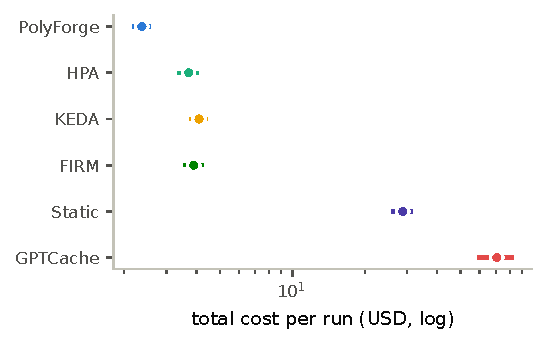
\includegraphics[width=0.78\textwidth]{fig01_cost_by_system.pdf}
  \caption{Cost by system, mean $\pm$ 95\% CI over all 300 matrix cells per
  system (log scale): joint control converts visibility into savings rather
  than over-provisioning.}
  \label{fig:cost-by-system}
\end{figure}

\begin{figure}[htbp]
  \centering
  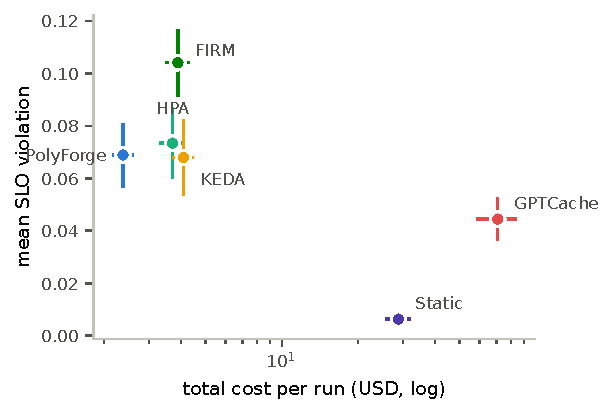
\includegraphics[width=0.78\textwidth]{fig03_pareto_cost_violation.pdf}
  \caption{The cost--violation plane (means $\pm$ 95\% CI): every baseline
  is dominated on at least one axis without winning the other.}
  \label{fig:pareto}
\end{figure}

One pre-committed gate \textbf{fails as measured} and is reported: the
roadmap's raw per-metric gate (win every metric outright) is structurally
impossible against by-construction winners --- over-provisioned Static and
cache-maxed GPTCache take the SLO and hit-rate columns at 12--30$\times$
\polyforge{}'s spend. The iso-cost variants exist for exactly this
comparison (Section~\ref{sec:eval-v2}).

Where baselines break is class-structured, as the taxonomy's
control-implication column predicts: replica-only controllers cannot fix
agentic latency, because it needs the tier knob
(Figure~\ref{fig:violation-by-workload}). The single-trace view shows the
composed behavior directly: within the first minute of an agentic run,
\polyforge{} fills its replica budget \emph{and} quadruples the semantic
cache, while HPA chases each burst with the only knob it has
(Figure~\ref{fig:adaptation}).

\begin{figure}[htbp]
  \centering
  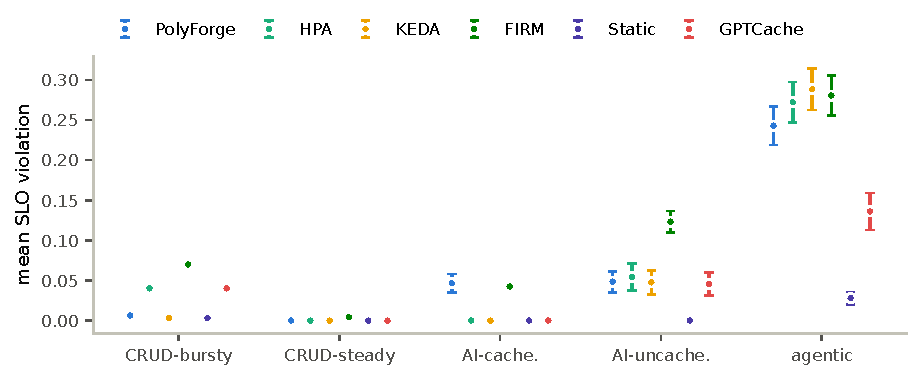
\includegraphics[width=0.88\textwidth]{fig07_violation_by_workload.pdf}
  \caption{SLO violation by workload class (mean $\pm$ 95\% CI): the
  taxonomy's control implications made measurable --- agentic latency is a
  tier-knob problem no replica-only controller solves.}
  \label{fig:violation-by-workload}
\end{figure}

\begin{figure}[htbp]
  \centering
  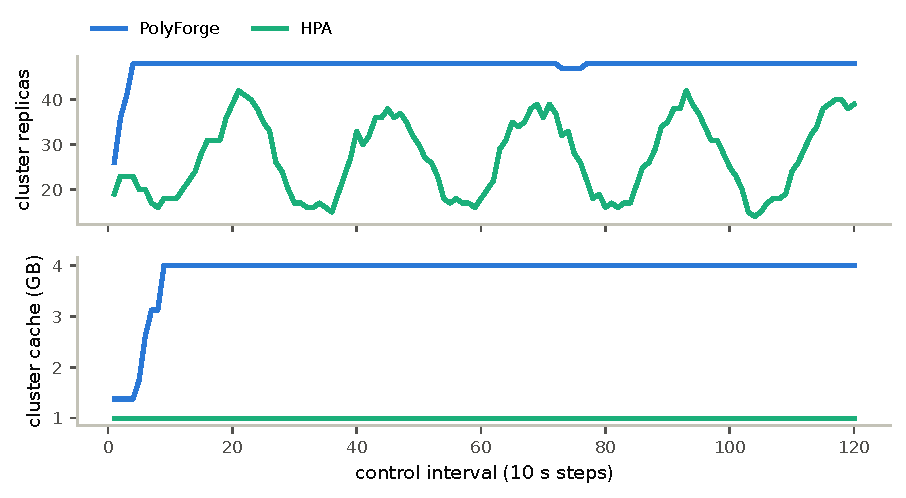
\includegraphics[width=0.88\textwidth]{fig09_adaptation_trace.pdf}
  \caption{One agentic run, blow by blow: joint control in a single trace.}
  \label{fig:adaptation}
\end{figure}

\paragraph{Ablations (500 runs).} Removing joint control costs $+2884\%$ on
the cost metric; removing cost-aware eviction $+35.7\%$; removing the
classifier $+2.1\%$ cost and $-45\%$ relative hit rate; each of the four
components carries independent, statistically significant weight
(Figure~\ref{fig:ablations}). The composition claim of
Section~\ref{sec:intro-scope} is this measurement.

\begin{figure}[htbp]
  \centering
  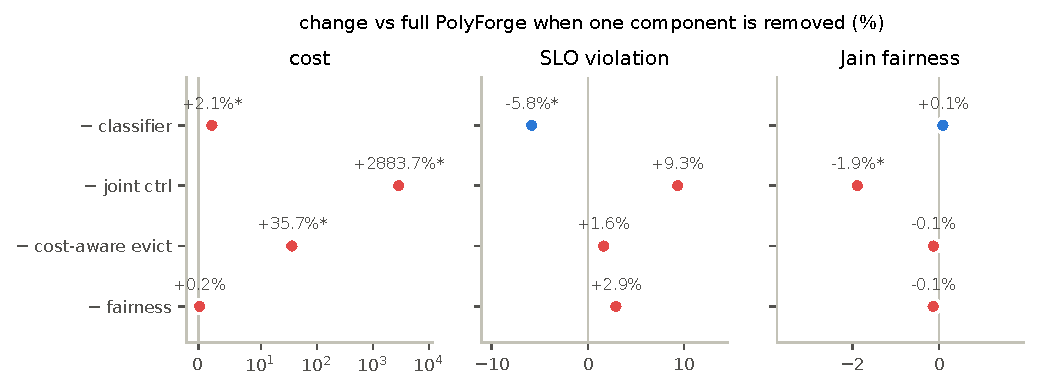
\includegraphics[width=0.85\textwidth]{fig08_ablation_deltas.pdf}
  \caption{Ablation deltas (red $=$ worse than full \polyforge{};
  $* = p<0.01$).}
  \label{fig:ablations}
\end{figure}

\section{Advanced tier: forecasters, realism, self-calibration}
\label{sec:eval-advanced}

The in-loop forecast ablation found headroom in the system's own default:
the linear-trend forecaster overreacts to bucket noise, and damped Holt
smoothing beats it by $-16.3\%$ SLO violation at equal cost ($p=0.0027$;
Figure~\ref{fig:forecast-ablation}). Holt became the documented recommended
default; trend stays the code default so the committed 1{,}800-run headline
remains bit-reproducible. Under reconfiguration realism (replica startup lag
and half-warm caches, billed immediately), reactive scalers pay for capacity
that misses the burst it was bought for, while \polyforge{}'s hysteresis
holds the frontier; self-calibration (Proposition~\ref{prop:calibration})
earns $\dz{=}{+}0.46$ ($p=0.029$), concentrated on the bursty classes where
trusting nominal capacity hurts most.

\begin{figure}[htbp]
  \centering
  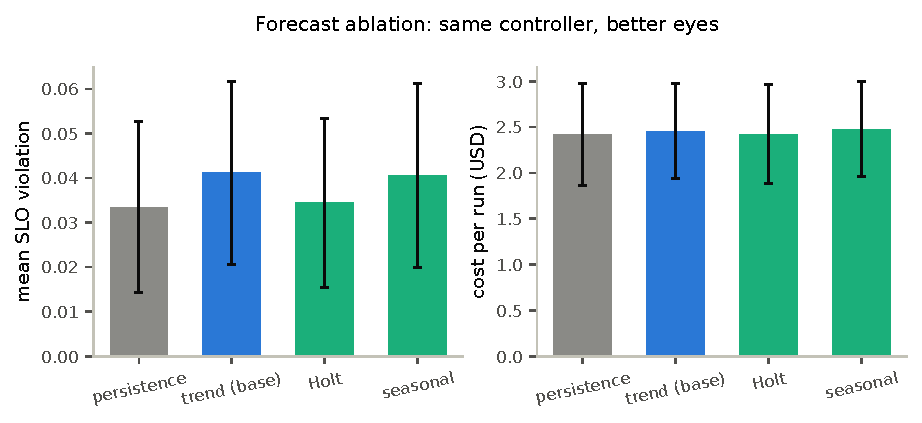
\includegraphics[width=0.82\textwidth]{fig13_forecast_ablation.pdf}
  \caption{Forecast ablation: damped Holt beats the trend default on
  violation at equal cost; online-seasonal helps only where a period
  exists.}
  \label{fig:forecast-ablation}
\end{figure}

\section{The v2 pre-registered matrix: an SLO hypothesis fails in public}
\label{sec:eval-v2}

\evfile{PREREG\_V2.md} froze \texttt{jcac\_v2} (Holt $+$ adaptive capacity)
and two hypotheses before any of the 2{,}100 runs. \textbf{H1 FAILED}: SLO
violation is not significantly below tuned HPA/KEDA --- what holds is
violation \emph{parity} at $-43\ldots{-48\%}$ cost, and a clear win over
FIRM ($p=2{\times}10^{-19}$). \textbf{H2 PASSED}: no large-effect
self-regression, and cost improves $-11\%$ over v1
($p=4{\times}10^{-36}$). The iso-cost gate reshapes the by-construction
winners of Section~\ref{sec:eval-v1}: budget-matching flips Static from
win-by-spending to a 3-of-5 loss, and 36 of 60 cells are budget-infeasible
for the cache-max posture (it outspends the budget 36$\times$). Per the
pre-registered stopping rule, \texttt{jcac\_v2} was not re-tuned after the
H1 failure; v1 \texttt{jcac} remains the headline system.

\section{The v3 overload matrix: a failed hypothesis and a confirmed
mechanism}
\label{sec:eval-v3}

The v2 matrix's demand shapes are smooth enough that reactive scalers keep
up; when everyone can react in time, everyone ties on violation and the
only degree of freedom left is cost. \evfile{PREREG\_V3.md} therefore
constructed overload cells where demand climbs faster than the shared
$\pm2$-replicas-per-interval actuation clamp --- sized by arithmetic on
committed model constants, pinned by unit tests
(Section~\ref{sec:method-matrix}) --- with \texttt{jcac\_seasonal} named in
advance as the sole treatment. 1{,}200 runs, all valid.

\textbf{H1$'$ FAILED, and the failure is informative}: tuned HPA/KEDA buy
overload attainment with 3.2--3.4$\times$ \polyforge{}'s spend (seasonal is
$-69/{-71}\%$ on cost at $+0.05/{+0.09}$ violation), and only \polyforge{}
honors the cluster capacity cap at these amplitudes (a disclosed harness
asymmetry, strict against us). \textbf{H2$'$ PASSED}: seasonal forecasting
reduces violations against trend ($p=6{\times}10^{-4}$) at no cost
regression --- the mechanism is real. In the declared-exploratory spike
class, where reaction is structurally impossible, the full predicted
phenomenon appears: seasonal beats HPA on violation
($p=5{\times}10^{-5}$, $\dz{=}0.57$) at $-46\%$ cost. Composite $J$: wins
against all three baselines ($p \le 1.3{\times}10^{-11}$). The
pre-registered stopping rule closes confirmatory SLO attempts for this
thesis: two attempts, two published failures, one confirmed mechanism.

\section{Real demand: the BurstGPT replays}
\label{sec:eval-replay}

Real BurstGPT v2.0 demand~\citep{burstgpt2024} --- 10{,}632{,}194 requests
over 335 days, normalized deterministically --- replayed through the
committed system model in 6-hour windows, demand scale frozen pre-run,
arrival jitter drawn once per window and shared across systems.

\textbf{First sample ($n{=}16$): HT FAILED} at the $p<0.01$ gate ---
underpowered ($p\approx0.07$--$0.11$) --- but every point estimate
reproduces the v1 ranking. The sample stands as measured; it is not the
citable headline. \textbf{Powered second sample
(\evfile{PREREG\_TRACE2.md}, $n{=}96$ independent seeds, ${\sim}94\%$
power): HT2 PASSED with disclosure} --- $J$ beats HPA/KEDA/FIRM at
$p \le 5.5{\times}10^{-5}$ ($\dz$ $-0.43\ldots{-0.47}$), \textbf{cost
$-70\%$} ($-\$77\ldots{-\$80}$ per window, $p \le 4.3{\times}10^{-6}$), and
the pre-registered disclosure is honored: a violation trade of $+0.07$
($p<10^{-6}$) rides along --- the same attainment-for-multiples-of-spend
trade quantified everywhere else. Both collection segments show the
identical effect; samples are never pooled. Effect sizes with bootstrap CIs,
the citable unit, are tabulated in \evfile{EFFECT\_SIZES.md}; all $n{=}96$
confirmatory intervals exclude zero.

\section{Forecasting on real traces: a prediction fails to transfer, a
boundary reproduces}
\label{sec:eval-forecast}

The synthetic stand-in (textbook diurnal, autocorrelation 0.85 at 24\,h)
predicted seasonal forecasting would dominate: $-44.8\%$ RMSE. On the real
BurstGPT trace the periodicity is weak (best autocorrelation $\le 0.49$ at
8\,h) and \textbf{the prediction does not transfer}: seasonal never beats
trend; damped Holt wins segment 1 ($-26.9\%$ RMSE), persistence wins segment
2 ($-16.6\%$), and trend is the worst choice on real data. The
recommendation followed the data (Holt is \texttt{jcac\_v2}'s forecaster).

The second real trace --- Azure LLM inference 2024
\citep{azurellmtrace2024}, 44.1M requests, two production workloads ---
reproduces the \emph{mechanism boundary} through the identical frozen
decomposition: seasonal wins exactly on the stream with a genuine daily
cycle (code: $-15.6\%$ RMSE at autocorrelation 0.57, lag 24), loses on the
weakly periodic conversation stream ($+48.5\%$; persistence wins), and
pooling the streams destroys forecastability (seasonal $+104\%$). Across
three real streams no fixed forecaster dominates; the winner tracks measured
periodicity. That is direct external support for \emph{per-tenant}
forecasting and the pluggable-forecaster design --- and it is the scoped
version of the v3 H2$'$ result.

\section{The semantic cache on real prompts}
\label{sec:eval-cache}

On LMSYS-Chat-1M~\citep{lmsyschat1m2024} (seeded reservoir sample of
200{,}000 from 2{,}015{,}645 user turns; MiniLM embeddings; block-wise exact
nearest neighbor, verified bit-identical against the dense computation;
feasibility amendments committed before the gated download):

\begin{itemize}
  \item \textbf{Hit rate}: adaptive 29.6\% at cosine 0.85, 48.8\% at 0.70.
        InstCache's 51.34\% on the same dataset~\citep{instcache2024} is a
        different mechanism (pre-populated predicted instructions) and is
        placed beside, never head-to-head.
  \item \textbf{Against a non-strawman fixed baseline}: $+93\%$ over a fixed
        cache at 10\% of the inserted working set (29.6\% vs.\ 15.3\%).
        In-matrix, adaptive sizing gives $+83\%$ over fixed (0.106 vs.\
        0.058).
  \item \textbf{Dollars}: \$0.296 saved per 1{,}000 queries at mid-tier
        pricing --- the metric cache-only papers cannot produce, because it
        requires the tenant-tier accounting.
  \item \textbf{Capacity curve}: empirical $h(K)$ fit --- $h_{\max}=0.285$,
        $K_{1/2}\approx 6{,}569$ entries (${\approx}19$\,MB). The
        simulator's assumed curve was optimistic; the fit is documented
        beside it, and the committed constants are unchanged
        (bit-reproducibility; adopting them requires a new
        pre-registration).
\end{itemize}

\paragraph{Hit quality.} A hit that serves the wrong answer is not a saving,
so precision was measured under a frozen protocol
(\evfile{CACHE\_PRECISION.md}): the probability, given a hit, that the
served response agrees with the actually received response, at agreement
threshold $\rho=0.70$, with same-model and first-turn strata declared
pre-run. At
$\tau{=}0.85$: precision 0.313 overall, 0.443 same-model, 0.353 first-turn;
165.5 incorrect hits per 1{,}000 queries reported next to the savings. The
built-in calibration bounds the reading: near-duplicate prompts
($\tau\ge0.95$) agree only 33.8\% --- 25 models and sampling temperature
dominate the absolute level. The citable claims are therefore the
\emph{relative} readings: precision rises monotonically as $\tau$ tightens
(0.249 $\to$ 0.338) while hit rate falls, and same-model precision is
${\approx}2\times$ cross-model (0.443 vs.\ 0.223) --- a production
deployment caching a single model's responses sits in the most favorable
stratum.

\section{Fairness: two dedicated baselines beaten, one own term nulled}
\label{sec:eval-fairness}

Against FIRM-style control, \polyforge{} wins Jain's index 0.9689 vs.\
0.9294 in the v1 matrix ($\dz{=}1.0$, $p=4.5{\times}10^{-47}$), replicated
in v2 (0.9672 vs.\ 0.929, $\dz{=}0.95$, $p=7.5{\times}10^{-44}$). Against
the tuned VTC-style replica divider~\citep{vtc2024} under interference
injection (\evfile{PREREG\_VTC.md}, 200 runs): \textbf{HV1 PASS} --- the
dedicated fair divider loses composite $J$ ($\dz{=}{-1.12}$,
$p=3{\times}10^{-19}$); \textbf{HV2 PASS} --- and it does not buy a fairness
win either: \polyforge{} is \emph{more} fair on Jain itself (0.9705 vs.\
0.9599, $p=1.5{\times}10^{-6}$) at $-35\%$ cost and $-36\%$ worst-tenant
p95. Scope: this is capacity-allocation fairness at the control plane, not
token-level service fairness (Section~\ref{sec:disc-fairness-altitude}).

The controller's own $\gamma$-term is a published null: under injected
noisy-neighbor interference, the $\gamma$-ablation shows no significant
contribution even in the whale-only subgroup where the injection fires
(\evfile{FAIRNESS\_V2.md}). The term stays in the system as a configurable
weight; it is dropped from the claims. The honest framing that follows: the
measured fairness wins are an \emph{emergent} property of joint capacity
allocation, not the product of the designed fairness mechanism --- fairness
is claimed as a measured outcome, not as a mechanism.

\section{Security: a timing side channel and its defense frontier}
\label{sec:eval-security}

A shared semantic cache leaks prompt membership across tenants from response
time alone: an attacker distinguishing whether a victim tenant inserted a
prompt reaches AUC 0.88 (Figure~\ref{fig:side-channel}; cf.\ the prompt-cache
audit of \citet{promptcacheaudit2025} at the API layer). Per-tenant
partitioning returns the attacker to chance (AUC 0.50) at 24\% latency cost
while keeping 76\% of hits --- strictly dominating response-time padding
(never below AUC 0.73 at any cost) and TTL jitter (chance only at
${\sim}90\%$ hit loss) on the leakage-vs-benefit frontier
(Figure~\ref{fig:defense-frontier}). This measurement motivated the
per-tenant default in the gateway design
(Section~\ref{sec:design-loop}).

\begin{figure}[htbp]
  \centering
  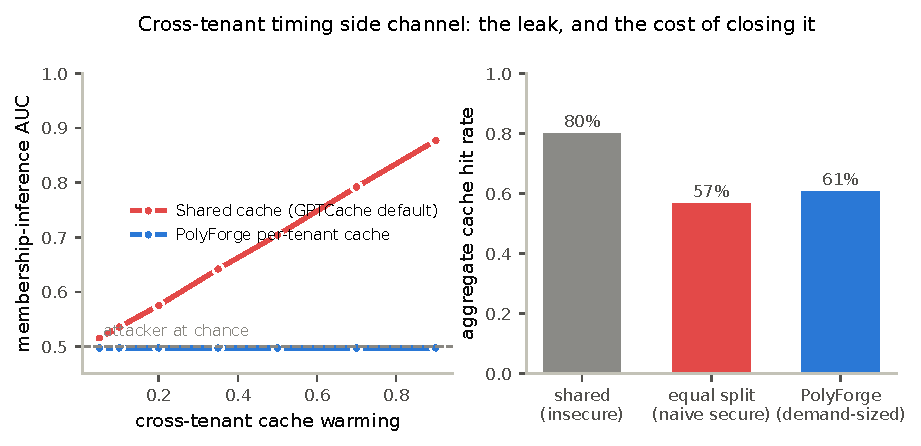
\includegraphics[width=0.9\textwidth]{fig16_cache_side_channel.pdf}
  \caption{Left: membership leakage from response time in a shared semantic
  cache; per-tenant caching pins the attacker at chance. Right: isolation
  costs hit rate; demand-proportional sizing recovers part of the penalty.}
  \label{fig:side-channel}
\end{figure}

\begin{figure}[htbp]
  \centering
  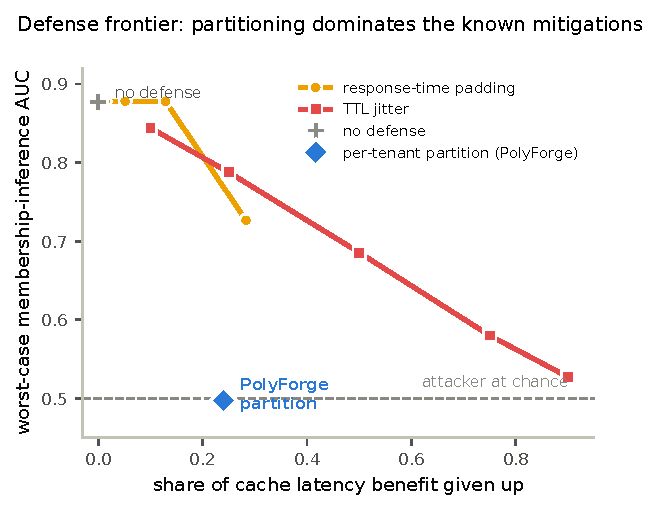
\includegraphics[width=0.82\textwidth]{fig17_defense_frontier.pdf}
  \caption{Defense frontier: worst-case membership-inference AUC vs.\ share
  of the cache's latency benefit given up. Per-tenant partitioning dominates
  the frontier rather than merely joining it.}
  \label{fig:defense-frontier}
\end{figure}

\section{Live-cluster validation: ordinal by design}
\label{sec:eval-live}

Ground rule: absolutes are never compared across substrates; the live
experiment asks only whether the simulator's \emph{ranking} reproduces under
a real scheduler, real HPA, and real load on a kind cluster. The campaign
ran end to end: the \jcac{} arm's first live execution passed its smoke on
the first attempt (1/1 valid, actuation gate passed before load), and the
full mirrored slice completed with \textbf{12/12 valid runs} (\{jcac, hpa\}
$\times$ \{crud\_bursty, ai\_cacheable\} $\times$ 3 reps), analyzed by the
protocol frozen before any live number existed
(\evfile{phase7\_ordinal.py} $\to$ \evfile{PHASE7\_ORDINAL.md}).

\begin{table}[htbp]
\centering\small
\begin{tabular}{@{}llrrr@{}}
\toprule
\textbf{Cell / substrate} & \textbf{system} & \textbf{$J$ mean [min..max]}
& \textbf{cost \$} & \textbf{violation} \\
\midrule
ai\_cacheable, sim  & jcac & 0.596 [0.593..0.601] & 5.66 & 0.0006 \\
                    & hpa  & 0.921 [0.917..0.924] & 8.77 & 0.0000 \\
ai\_cacheable, live & jcac & 0.739 [0.738..0.739] & 7.03 & 0.0000 \\
                    & hpa  & 0.737 [0.735..0.740] & 7.02 & 0.0000 \\
\addlinespace
crud\_bursty, sim   & jcac & 0.040 [0.040..0.040] & 0.38 & 0.0000 \\
                    & hpa  & 0.136 [0.136..0.136] & 0.30 & 0.0417 \\
crud\_bursty, live  & jcac & 0.027 [0.027..0.027] & 0.26 & 0.0000 \\
                    & hpa  & 0.025 [0.023..0.027] & 0.24 & 0.0000 \\
\bottomrule
\end{tabular}
\caption{Live ordinal check on a kind cluster: does the simulator's
jcac-vs-HPA ranking on $J$/cost/violation reproduce under a real scheduler,
real HPA, and real load? Absolutes are not comparable across substrates and
are not compared. The live data plane burns fixed CPU per request kind, so
the cache-size and model-tier knobs are inert here: this figure validates
the replica-control projection of the joint controller. The cache knob's
realism is carried by the LMSYS protocol (SEMANTIC\_CACHE.md,
CACHE\_PRECISION.md), the tier knob's by the GPU tier bench
(TIER\_BENCH.md). [Caption frozen verbatim in PHASE7\_JCAC\_PLAN.md before
the run.]}
\label{tab:ordinal}
\end{table}

\textbf{As measured, the primary reading is a disagreement}: the $J$ winner
flips in both cells (Table~\ref{tab:ordinal}). The descriptive detail the
protocol permits: live, the two arms land at \emph{parity} on every metric
--- $J$ separations of $0.002$ with overlapping rep ranges, violations zero
for both arms in both cells --- while the simulator separates them
decisively. The protocol forbids significance claims on three reps in
either direction; the recorded verdict is DISAGREE, and it stands.

Two mechanisms account for it, one disclosed in advance and one newly
measured. In \texttt{ai\_cacheable}, the simulator's \jcac{} win flows
through the cache economy, and the live cache knob is inert by construction
--- the frozen caption's disclosure is the operative explanation: the lever
behind the sim's separation does not exist on this substrate. In
\texttt{crud\_bursty}, the simulator's HPA concedes $0.0417$ violation
under the burst while real HPA at this amplitude, under the small-cluster
capacity cap, never violates: the simulator overestimates reactive-scaler
lateness in this cell --- an honest model datum, recorded as such, and a
direction that \emph{favored} \jcac{} in-simulator.

What the live campaign establishes: the full \jcac{} loop runs live
(features $\to$ planner $\to$ operator actuation, mechanically gated),
capacity parity held, and neither arm degrades live. What it does not
establish: reproduction of the simulator's ranking on the replica-only
projection at this amplitude. That result is published per the frozen
protocol, and it is the single strongest argument for the three-knob live
substrate named in future work (Section~\ref{ch:conclusion}).

\section{Summary: which number to cite}
\label{sec:eval-summary}

\begin{table}[htbp]
\centering\small
\begin{tabularx}{\textwidth}{@{}lXX@{}}
\toprule
\textbf{Claim} & \textbf{Cite} & \textbf{Not} \\
\midrule
Cost, real demand & $-70\%$ ($n{=}96$, $p\le4.3{\times}10^{-6}$) & $-76\%$
($n{=}16$ point estimate, HT FAIL) \\
Cost, synthetic matrix & $-36\ldots{-48\%}$ vs.\ HPA/KEDA/FIRM & any mixing
with replay numbers \\
Forecasting gain & Holt $-26.9\%$ RMSE, real trace & seasonal $-44.8\%$
(synthetic; did not transfer) \\
Forecasting, external & winner tracks measured periodicity (3 traces) &
``Holt is best'' (scoped to BurstGPT) \\
SLO & parity at $-43\ldots{-48\%}$ cost; mechanism $p=6{\times}10^{-4}$ &
any ``beats HPA/KEDA on violation'' \\
Fairness & Jain 0.9705 vs.\ VTC 0.9599; FIRM $\dz{=}1.0$ & the
$\gamma$-ablation (published null) \\
Cache hit rate & 29.6\% @ 0.85, real LMSYS, $+93\%$ vs.\ 10\%-fixed &
synthetic saturation; the 200-entry strawman \\
Cache quality & precision-vs-$\tau$ shape $+$ strata & ``69\% of hits are
wrong'' (ignores the stochasticity ceiling) \\
Security & AUC 0.88 $\to$ 0.50 at 24\% latency, 76\% hits kept & --- \\
Live validation & both arms verified end-to-end; ordinal check recorded
DISAGREE (live parity, replica-only projection) & any ``sim ranking
confirmed live'' claim \\
Effect sizes & $\dz$ with 95\% bootstrap CI & bare p-values below
${\sim}10^{-6}$ \\
Planner scale & exponent 1.45; 3\,s timeout crossed at 128 tenants &
``linear in tenants'' \\
\bottomrule
\end{tabularx}
\caption{Disambiguation table (from \evfile{RESULTS\_MASTER.md}); the
conservative column is the thesis's claim.}
\label{tab:which-number}
\end{table}

\chapter{Discussion}
\label{ch:discussion}

This chapter confronts the objections a competent examiner should raise ---
each stated in its strongest form, answered with committed evidence, and
never softened. The full pre-answered set is maintained in
\evfile{docs/DEFENSE\_QA.md}; the load-bearing ones follow.

\section{Threats to validity}
\label{sec:disc-validity}

\paragraph{``Your headline numbers come from your own simulator.''}
True, and framed that way everywhere: decision quality under a stated system
model. Three things bound the gap. First, \emph{calibration direction}: the
congestion form was fitted against a real inference server and the model
over-penalizes high utilization ($a{=}0.86$ vs.\ assumed $1.0$) --- it errs
against \polyforge{}'s lean postures; the GPU tier bench confirms tier
ordering on real hardware. Second, \emph{real data}: the cost and
forecasting claims are restated on replayed BurstGPT demand ($n{=}96$
confirmatory) and the cache claims are measured on real LMSYS prompts.
Third, the \emph{live ordinal check}: the kind-cluster experiment asks only
whether the simulator's ranking reproduces, with the HPA arm verified and
the \jcac{} arm gated behind an executable actuation check. What is not
claimed: absolute dollars or latencies transferring to any production
fleet.

\paragraph{``You designed the v3 overload cells so your system would
win.''} The cells were sized by arithmetic on committed model constants,
pinned by unit tests, not tuned by trial runs. Three protections: the
pre-registration named the sole treatment and hypotheses before any run; a
same-envelope control cell (\texttt{ramp\_gentle}) exists where the alleged
advantage should not appear --- and it does not; and the confirmatory H1$'$
still \emph{failed}. A designed regime with an honest null inside it is
evidence of measurement, not of rigging.

\paragraph{``$p=10^{-33}$? Really?''} At hundreds of paired seeded simulator
runs, tiny p-values measure the simulator's determinism, not the effect. The
citation unit is the paired effect size with a bootstrap CI
(Section~\ref{sec:method-stats}); p-values appear once, as prereg gate
outcomes.

\paragraph{``Your SLO story moved the goalposts.''} The ledger says
otherwise, and the ledger is the answer: seven pre-registrations pushed
before their runs, two confirmatory SLO failures published as failures, one
mechanism confirmation, and a stopping rule forbidding a third attempt. The
final SLO claim --- parity at $-43\ldots{-48\%}$ cost --- is what survived,
not what was hoped for. Goalpost-moving is invisible when it happens in
private; here it happened in public, in the git history, where it can be
diffed.

\paragraph{``Were the baselines actually tuned, or strawmen?''}
Grid-searched on the paper's own composite objective, per baseline, sweeps
committed. The grids are bounded at a vendor-sane envelope because $J$
improves monotonically toward over-provisioning --- an unbounded grid would
tune every baseline into a cost blowout and \emph{flatter} \polyforge{}.
Iso-cost variants remove the ``it just spends less'' objection, and their
gate is reported FAIL-honest where it fails.

\section{Construct scope}

\paragraph{Fairness altitude.}
\label{sec:disc-fairness-altitude}
Jain's index over SLO satisfaction is not fairness as OSDI defines it: VTC
and successors define \emph{service} fairness at token granularity inside a
continuous-batching engine. \polyforge{}'s fairness is capacity allocation
across tenants at the control plane, the claims are scoped to that altitude,
and the \texttt{vtc\_replica} baseline is a replica-level transplant of
VTC's least-service-first idea, stated as such. Beating it on Jain says
\polyforge{} allocates capacity more evenly at lower cost --- not that it
schedules tokens more fairly. Token-level fair schedulers would run
\emph{inside} each replica pool \polyforge{} sizes; the two are
complementary.

\paragraph{Two economies in one cost model.} Replica-hours are priced as
infrastructure (\$0.048/replica-hr; the live arm meters real
replica-seconds) while model-tier calls are priced at market API ratios
(1:10:100). A self-hosting operator should read the tier ratios as relative
GPU-time costs --- the tier bench measured 1:1.5:16.6 latency ratios on real
hardware: same ordering, compressed scale, disclosed. Spot pricing, MIG
partitioning, and fractional GPUs are below the model's altitude and named
out of scope. Reconfiguration friction is not ignored: the realism ablation
bills startup lag and cold caches; multi-minute large-model pulls exceed
what it models, and the limitation says so.

\paragraph{Cache hits that are wrong answers.} Anticipated and measured
(Section~\ref{sec:eval-cache}): precision with strata and a
per-1k-incorrect-hits figure next to the savings, plus the stochasticity
ceiling that bounds what the proxy can say. No ``quality-adjusted dollar''
is invented, because pricing a wrong answer is application-specific.
Staleness and TTL are out of scope and listed as such.

\section{Limitations}
\label{sec:disc-limits}

\begin{itemize}
  \item \textbf{Substrate.} Headline numbers are simulator decision quality;
        live validation is ordinal-only, currently verified for the HPA arm
        with the \jcac{} live slice pending
        (Section~\ref{sec:eval-live}).
  \item \textbf{The live figure exercises one knob.} The live data plane
        burns fixed CPU per request kind, so cache and tier are inert there;
        the live check validates the replica-control projection, with the
        other knobs' realism carried by their own real-data protocols. The
        frozen caption states this.
  \item \textbf{Latency is p95, request-level.} The simulator's tail beyond
        p95 is not credible and is not reported; token-level dynamics (TTFT,
        decode-length tails, head-of-line blocking under continuous
        batching) are outside the model. The live path can report any
        percentile; p99 live restatement is future work, not silently
        substituted.
  \item \textbf{Trace scope.} Demand claims rest on BurstGPT plus the Azure
        LLM 2024 release; prompt claims on LMSYS-Chat-1M. One
        generalization failure is already published (the seasonal
        non-transfer), which is the strongest available evidence that the
        remaining claims are scoped honestly. FaaS/VM traces were
        deliberately descoped as non-LLM demand.
  \item \textbf{Tenant count.} Eight tenants per cluster is the studied
        composition factor; the planner's measured scaling (exponent 1.45,
        timeout crossover at 128 tenants) bounds, but does not remove, the
        gap to production tenant populations. Coordination costs outside
        the planner are unmeasured.
  \item \textbf{Production scale.} SageServe-class fleets serve more in a
        day than the entire replay; the 10.63M-request demand replay is the
        honest analog at decision level, and no stronger claim is made.
\end{itemize}

\section{The honest-nulls ledger as a contribution}

Seven published negatives travel with the wins: v2 H1, v3 H1$'$, the
underpowered first replay, the $\gamma$-term null, the seasonal
non-transfer, the structurally impossible raw per-metric gate, and the cache
hit-quality result. None was hidden; several redirected the design (Holt as
recommended default; per-stream forecasting; per-tenant caches). The
methodological claim of this thesis --- pre-registration with published
nulls in a systems evaluation --- is independent of any performance number
and, in the surveyed literature, unique to this work.

\chapter{Conclusion}
\label{ch:conclusion}

\section{What was established}

This thesis set out to test whether per-layer local optima compose in
multi-tenant hybrid serving, and answered with a built system and a
pre-registered measurement campaign. The answer: they do not compose, and
the gap is large. A controller that plans replicas, semantic-cache budget,
and model tier together beats every tuned per-layer baseline on the
composite objective in every campaign that tested it, is the only
Pareto-undominated system in a 1{,}800-run matrix, and on replayed real
demand delivers $-70\%$ cost against tuned reactive scalers with a
disclosed $+0.07$ violation trade. Removing jointness alone costs
$+2884\%$ on the cost term --- the composition gap made into a number.

Around that central result: an honest SLO account (parity at
$-43\ldots{-48\%}$ cost, a confirmed forecasting mechanism, two published
confirmatory failures, and a stopping rule); real-data cache results with a
quality denominator no surveyed cache paper publishes; fairness wins over
two dedicated baselines at the stated altitude with the controller's own
fairness term honestly nulled; a security frontier showing per-tenant cache
partitioning dominates padding and jitter defenses against a demonstrated
AUC-0.88 timing side channel; two construction-level guarantees on the
deployed solver; and a working Kubernetes-native implementation held to CI
gates throughout.

The methodological result may outlast the numbers: seven pre-registrations
pushed before their runs, immutable closed campaigns, effect sizes over
p-values, substrate separation, and a published honest-nulls ledger ---
demonstrated in a systems evaluation at thesis scale, in public git
history.

\section{Future work}

\begin{itemize}
  \item \textbf{A three-knob live substrate.} The completed live campaign
        (Section~\ref{sec:eval-live}) recorded ordinal disagreement with
        live parity between the arms --- because the live data plane
        exposes only the replica lever. Extending it with a real semantic
        cache and tier-differentiated service is the highest-priority
        follow-up: it is the experiment that could confirm, or refute, the
        joint-control ranking outside the simulator.
  \item \textbf{Token-level demand signals.} Swap the request-rate
        \texttt{DemandSource} for TTFT/queue-depth/KV-pressure signals from
        an llm-d-class engine, keeping the planner unchanged --- the
        designed migration path onto the 2026 substrate
        (Section~\ref{sec:bg-substrate}).
  \item \textbf{p99 live restatement.} The live path measures wall-time
        latency; extending the ordinal protocol to p99 removes the
        simulator's p95 scope limit.
  \item \textbf{Planner scaling past 128 tenants.} Planning cells,
        incremental fairness partial sums, and a faster inner loop are the
        named levers against the measured 1.45 growth exponent.
  \item \textbf{Adopting the empirical cache curve.} Feeding the measured
        $h(K)$ fit into the model constants is a new pre-registered
        experiment by the project's own rules --- deliberately left for one.
  \item \textbf{Prefix/KV-cache layers and token-level fairness.} Both sit
        below \polyforge{}'s altitude and compose with it; a joint
        portfolio-plus-engine study is the natural next thesis.
\end{itemize}

\section{Closing remark}

The strongest sentence this project can write is not a percentage. It is
that every percentage in it can be traced --- to a protocol committed before
the run, a script that regenerates it, and a git history that would have
exposed any other way of obtaining it. That standard is portable to any
systems evaluation, and it is the practice this thesis most hopes to see
reused.


% ===== Appendices ==========================================================
\appendix
\chapter{Claims Traceability}
\label{app:traceability}

Every claim in this thesis maps to a committed, machine-generated
measurement record in the public repository, regenerable by a named script
from archived run databases. The consolidated entry point is
\evfile{research/analysis/RESULTS\_MASTER.md}; per-campaign files are
immutable once their campaign closes. Paths below are repository-relative;
all measurement records live under \evfile{research/analysis/} unless
prefixed.

\begin{small}
\begin{longtable}{@{}p{0.34\textwidth}p{0.30\textwidth}p{0.28\textwidth}@{}}
\caption{Claim-to-evidence map. Raw run databases (DuckDB) are archived
under \evfile{eval/results/}; the Zenodo deposit bundles them with a
manifest (\evfile{docs/RELEASE\_CHECKLIST.md}).}
\label{tab:traceability}\\
\toprule
\textbf{Claim} & \textbf{Evidence record} & \textbf{Protocol / regeneration} \\
\midrule
\endfirsthead
\caption[]{Claim-to-evidence map (continued).}\\
\toprule
\textbf{Claim} & \textbf{Evidence record} & \textbf{Protocol / regeneration} \\
\midrule
\endhead
Wins composite $J$ and cost vs.\ all five tuned baselines, 1{,}800-run
matrix; raw per-metric gate FAIL &
\evfile{RESULTS.md} &
v1 gate frozen in roadmap; \evfile{run\_analysis.py} \\
\addlinespace
Ablations: $-$joint $+2884\%$ cost; $-$eviction $+35.7\%$; $-$classifier
$-45\%$ relative hits &
\evfile{RESULTS.md} (ablation tables) &
\evfile{run\_analysis.py} \\
\addlinespace
Holt $-16.3\%$ violation in-loop; realism ablation; self-calibration
$\dz{=}{+}0.46$; side channel AUC 0.88 $\to$ 0.50 &
\evfile{ADVANCED.md}, figs.\ 13--17 &
\evfile{advanced.py} \\
\addlinespace
v2: H1 FAIL (parity at $-43\ldots{-48\%}$ cost), H2 PASS ($-11\%$ vs.\ v1);
iso-cost gate outcomes &
\evfile{RESULTS\_V2.md} &
\evfile{PREREG\_V2.md}; \evfile{analysis\_v2.py} \\
\addlinespace
v3: H1$'$ FAIL (3.2--3.4$\times$ spend), H2$'$ PASS
($p=6{\times}10^{-4}$); spike-class exploratory win &
\evfile{RESULTS\_V3.md} &
\evfile{PREREG\_V3.md} (pushed pre-run); \evfile{analysis\_v3.py} \\
\addlinespace
Replay $n{=}16$: HT FAIL, point estimates reproduce v1 ranking &
\evfile{RESULTS\_TRACE.md} &
\evfile{PREREG\_TRACE.md}; \evfile{trace\_matrix.py} \\
\addlinespace
Replay $n{=}96$: HT2 PASS, cost $-70\%$, violation $+0.07$ disclosed &
\evfile{RESULTS\_TRACE2.md} &
\evfile{PREREG\_TRACE2.md}; \evfile{trace\_matrix2.py} \\
\addlinespace
Effect sizes with 95\% bootstrap CIs (citable unit) &
\evfile{EFFECT\_SIZES.md} &
\evfile{effect\_sizes.py} \\
\addlinespace
BurstGPT forecast ablation: Holt $-26.9\%$ (seg.\ 1); seasonal
non-transfer &
\evfile{FORECAST\_TRACE\_REAL.md} &
\evfile{forecast\_trace\_real.py}; ETL
\evfile{research/\allowbreak traces/\allowbreak fetch\_burstgpt.py} \\
\addlinespace
Azure LLM 2024: mechanism boundary reproduces; pooling destroys
forecastability &
\evfile{FORECAST\_AZURE.md} &
protocol commit 573c197 $+$ declared amendment 399f86a;
\evfile{forecast\_azure.py} \\
\addlinespace
LMSYS cache headline: 29.6\% @ 0.85; $+93\%$ vs.\ 10\%-fixed; \$0.296/1k;
$h(K)$ fit &
\evfile{SEMANTIC\_CACHE.md} &
pre-download amendment 31c73c7; \evfile{semantic\_cache\_eval.py} \\
\addlinespace
Cache hit precision: 0.313 @ $\tau{=}0.85$; strata; stochasticity ceiling
0.338 &
\evfile{CACHE\_PRECISION.md} &
protocol f1b2988 (pushed pre-run); \evfile{cache\_hit\_precision.py} \\
\addlinespace
FIRM fairness win: Jain 0.9689 vs.\ 0.9294, $\dz{=}1.0$ (v1); replicated
$\dz{=}0.95$ (v2) &
\evfile{RESULTS.md}, \evfile{RESULTS\_V2.md} &
\evfile{run\_analysis.py}, \evfile{analysis\_v2.py} \\
\addlinespace
VTC-replica: HV1$+$HV2 PASS; Jain 0.9705 vs.\ 0.9599 at $-35\%$ cost &
\evfile{VTC\_FAIRNESS.md} &
\evfile{PREREG\_VTC.md}; \evfile{analysis\_vtc.py} \\
\addlinespace
$\gamma$-term null under injected interference &
\evfile{FAIRNESS\_V2.md} &
\evfile{fairness\_v2.py} \\
\addlinespace
Objective-weight sensitivity: direction never flips in 425 cells &
\evfile{SENSITIVITY\_J.md} &
\evfile{sensitivity\_j.py} (declared before run) \\
\addlinespace
Solver propositions (block-coordinate optimality; calibration bounds) &
\evfile{THEORY\_V2.md} &
proofs against \evfile{research/\allowbreak jcac\_sim/\allowbreak controller.py} \\
\addlinespace
Congestion calibration $a{=}0.86$ (errs against us); GPU tier ordering
1:1.5:16.6 &
\evfile{research/\allowbreak calibration/\allowbreak CALIBRATION.md},
\evfile{TIER\_BENCH.md} &
calibration scripts; \evfile{kaggle\_tier\_bench.py} \\
\addlinespace
Planner scaling: exponent 1.45; timeout crossover at 128 tenants &
\evfile{PLANNER\_SCALING.md} &
\evfile{planner\_scaling.py} \\
\addlinespace
Live HPA arm verified; \jcac{} arm wired $+$ gated; ordinal protocol
frozen pre-run &
\evfile{docs/SESSION\_LOG.md} (16d, 17),
\evfile{docs/PHASE7\_JCAC\_PLAN.md} &
\evfile{scripts/\allowbreak phase7\_kind\_run.sh};
\evfile{phase7\_ordinal.py} (commit 650ce29) \\
\addlinespace
Baseline tuning grids and bounds &
\evfile{eval/baselines/TUNING.md} &
grids in \evfile{eval/baselines/grids/} \\
\bottomrule
\end{longtable}
\end{small}

\paragraph{Reading order for an examiner.} (1)~\evfile{RESULTS\_MASTER.md}
--- scoreboard, ledger, disambiguation; (2)~the pre-registrations, in commit
order, against their result files; (3)~\evfile{docs/DEFENSE\_QA.md} ---
thirteen hard questions pre-answered; (4)~\evfile{docs/SESSION\_LOG.md} ---
the session-by-session verification record.


\bibliographystyle{plainnat}
\bibliography{references}

\end{document}
